\documentclass[tikz]{standalone}

\begin{document}
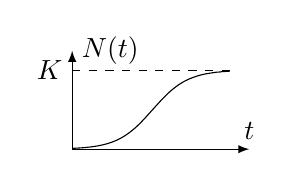
\begin{tikzpicture}
\draw[-latex] (0,0) -- (2.25,0) node [above] {\(t\)};
\draw[-latex] (0,0) -- (0,1.25) node [right] {\(N(t)\)};
\draw[dashed] (0,1) -- (2,1);
\node[left] at (0,1) {\(K\)};
\draw[domain=0:2, variable=\t, samples=100]
plot( {\t}, {0.01/(0.01 + 0.99*exp(-4.5*\t))});
\end{tikzpicture}
\end{document}
